% ALTA 2026 Shared Task system description. Build: latexmk -pdf main.tex
\documentclass[11pt]{article}
\usepackage[final]{acl}
\usepackage{times}
\usepackage{latexsym}
\usepackage[T1]{fontenc}
\usepackage[utf8]{inputenc}
\usepackage{microtype}
\usepackage{inconsolata}
\usepackage{booktabs}
\usepackage{amsmath}
\usepackage{array}
\usepackage{graphicx}
\usepackage{xcolor}
\usepackage{url}
\usepackage{enumitem}
\setlist{nosep,leftmargin=1.4em}
\newcommand{\pboot}{P_{\mathrm{boot}}}

\title{Two Varieties, Two Sarcasms: A Cross-Validated Ensemble and an Analysis\\of Australian and British Sarcasm Labels}

\author{Irving Ernesto Quezada Ram\'{i}rez \\
  Independent researcher \\
  \texttt{research@irvingernesto.com}}

\begin{document}
\maketitle

\begin{abstract}
We describe the system of team Stargazers (CodaBench user \texttt{thermostatic}) for the ALTA 2026 shared task: binary
sentiment and sarcasm classification of Australian (\mbox{en-AU}) and British (\mbox{en-UK}) English Google reviews and Reddit
comments, scored by averaging, over the two tasks, the lower of the two varieties' macro-F1. Our system averages a
fine-tuned DeBERTa-v3-large classifier and two logistic-regression probes on frozen model representations, selected
with five-fold cross-validation. It scored 0.867 on the test set, ranked second, and was one of six joint winners.
Doubling the training data or averaging more random seeds raises our two strongest models' scores by at most 0.004.
The two varieties' sarcasm labels, however, differ. Among Reddit comments that a sentiment classifier labels negative,
each en-AU subreddit has a higher share labelled sarcastic (44--64\%) than each en-UK subreddit (12--33\%). Classifier
scores for derision (mocking, contempt, anger, cynicism) are positively associated with the en-AU sarcasm label (mean
AUC 0.70) and inversely with the en-UK label (0.43). With one annotator per variety, we cannot attribute these
differences to the annotators, the communities or the texts.
\end{abstract}

\section{Introduction}
\label{sec:intro}

\begin{figure}[t]
\centering
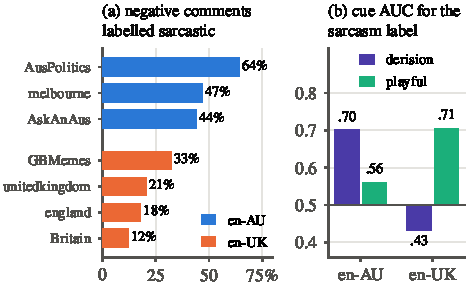
\includegraphics[width=\columnwidth]{fig_headline.pdf}
\caption{Sarcasm-label rates and cue associations differ between the en-AU and en-UK data. (a) Share of Reddit comments
labelled sarcastic by the dataset annotator, per subreddit, among comments that the SiEBERT sentiment classifier labels
negative and that we matched to the Arctic Shift archive (1,221 en-AU, 883 en-UK). (b) Mean ROC AUC of the four derision
cues and the four playful cues (\S\ref{sec:constructs}) for the annotator's sarcasm label, among all comments that
SiEBERT labels negative. AUC 0.5 is chance level; values below 0.5 indicate an inverse association. No panel uses the
LLM re-annotation of Appendix~\ref{app:readers}.}
\label{fig:headline}
\end{figure}

The ALTA 2026 shared task \citep{alta2026task} uses the Australian (en-AU) and British (en-UK) English portions of
BESSTIE, a benchmark for sentiment and sarcasm classification across varieties of English
\citep{srirag-etal-2025-besstie}. Each text is a Google review or a Reddit comment with two binary labels: sentiment
(positive or negative) and sarcasm (sarcastic or not). Each task is scored by macro-F1, the unweighted mean of the two
classes' F1 scores, computed separately for each variety. The official score takes the lower variety-level macro-F1 for
each task and averages these two values. We call the variety with the lower macro-F1 the \emph{binding} variety, because
only its score enters the official score. For example, our test macro-F1 scores of 0.932 (en-AU) and 0.976 (en-UK) for
sentiment and 0.801 (en-AU) and 0.837 (en-UK) for sarcasm give $(0.932+0.801)/2\approx0.867$.

This paper makes two contributions. First, it describes a three-member ensemble, selected with the protocol of
\S\ref{sec:protocol}, that ranked second and shared first place. Second, it shows that the en-AU and en-UK sarcasm labels
differ in their rates and in their associations with automatically scored cues. This matters for how the benchmark is
used: when a model trained on one variety scores lower on the other, part of the drop may reflect different labelling
conventions or different texts rather than the model's handling of the variety. Figure~\ref{fig:headline} summarises the
evidence: among comments labelled negative by a sentiment classifier, 44--64\% are labelled sarcastic in each en-AU
subreddit against 12--33\% in each en-UK subreddit, and contempt and anger scores are associated with the sarcastic label
in en-AU but with the non-sarcastic label in en-UK. These analyses describe where the labels differ; they do not identify
why the official score changes little across the configurations we tested.

Our findings are:
\begin{enumerate}
\item The ensemble scored 0.867 on the test set, ranked second, and was one of six joint winners (\S\ref{sec:results}).
\item From 50\% to 100\% of the training data, DeBERTa's score rises from 0.858 to 0.862 and the LLM probe's stays at
0.853; from three to ten DeBERTa seeds, the score rises from 0.863 to 0.864. Adding the two probes raises it by 0.006--0.007
(\S\ref{sec:capacity}).
\item Derision cues are associated with the sarcastic label in en-AU (AUC 0.66--0.73), whereas contempt and anger are
associated with the non-sarcastic label in en-UK (pooled AUCs 0.41 and 0.38; 0.33--0.47 within each en-UK subreddit)
(\S\ref{sec:constructs}).
\item BESSTIE reports human agreement of $\kappa=0.47$ for en-AU sarcasm; among Reddit comments labelled negative, our
ensemble's sarcasm AUC is 0.77 in en-AU against 0.91 in en-UK (\S\ref{sec:ceiling}).
\end{enumerate}
We also report interventions that did not meet our improvement criteria (\S\ref{sec:negative}) and an exploratory
re-annotation by a large language model (LLM) without access to the gold labels (Appendix~\ref{app:readers}).

\paragraph{Related work.} Two findings on sarcasm interpretation bear on ours: \citet{oprea-magdy-2020-isarcasm} show that
the sarcasm an author intends differs from the sarcasm readers perceive, and \citet{oprea-magdy-2020-sociocultural} relate
sarcasm interpretation to readers' country, age and whether English is their native language. BESSTIE extends
variety benchmarks such as DIALECTBENCH \citep{faisal-etal-2024-dialectbench} to sentiment and sarcasm in English
varieties, and its authors reported lower sarcasm performance when the training and evaluation varieties differ
\citep{srirag-etal-2025-besstie}. \citet{singh2025nekminit} add explanations to BESSTIE's Australian and Indian English
sarcasm data and evaluate a prompting method for explainable sarcasm detection. Our analysis concerns label variation and
annotator effects \citep{geva-etal-2019-modeling,basile-etal-2021-need,plank-2022-problem}. \citet{rottger-etal-2022-two}
distinguish descriptive annotation, which elicits annotators' own judgements, from prescriptive annotation, which asks
them to apply one specified interpretation. The EPIC study collected irony judgements from annotators in five
English-speaking countries, including the UK and Australia, and modelled the differences between these groups
\citep{frenda-etal-2023-epic}. In pragmatics, jocular mockery and abuse (remarks that appear hostile but are used
playfully, often to signal closeness) have been described in both Australian and British interaction
\citep{haugh2012mock}. Our contribution is specific to this benchmark: a system for the shared task, and an analysis of
how the two BESSTIE sarcasm label sets relate to automatically scored cues, conducted within each subreddit.

\section{Task and Data}
\label{sec:data}
The training and development files together (the \emph{pool}) contain 6,288 texts: 3,080 en-AU (1,076 reviews, 2,004
Reddit comments) and 3,208 en-UK (2,065 reviews, 1,143 comments). We call each variety--source combination a
\emph{segment}. Of the 1,163 texts labelled sarcastic, 1,089 (94\%) are Reddit comments: 42\% of en-AU and 22\% of en-UK
comments are labelled sarcastic, against 6.8\% of en-AU reviews and 1 of the 2,065 en-UK reviews. The test set contains
1,573 texts with the same segment proportions as the pool (270 en-AU reviews, 501 en-AU comments, 516 en-UK reviews,
286 en-UK comments).

BESSTIE selected Reddit comments from variety-specific subreddits and Google reviews of places in each country, so the
variety tags are dataset assignments, not verified speaker identities; annotators discarded texts they judged to
express no clear positive or negative sentiment. One annotator labelled each variety, and a second annotator labelled 50
items per variety for an agreement study. The guideline reads: ``Annotate if the comment uses irony or mockery to express
contempt or ridicule,'' and asks annotators to ``consider the tone and context of the comment''
\citep{srirag-etal-2025-besstie}. We see two possible readings: an inclusive one, in which literal mockery that expresses
contempt or ridicule counts as sarcasm, and a narrower one, which requires non-literal (ironic) meaning.
Table~\ref{tab:examples} shows examples of both readings.

The official split assigns individual Reddit comments, not whole threads, to the training and development files. We
matched 95\% of the Reddit texts (95.0\% en-AU, 95.9\% en-UK) to the Arctic Shift archive of public Reddit comments
\citep{arcticshift}. The matched comments come from seven subreddits and were posted between 18 February and 2 June
2024, and 82\% of the matched development comments share a thread with a training comment. With cross-validation folds
that keep each thread in one fold, the ensemble's score (with DeBERTa averaged over three seeds) falls by 0.0012, from
0.8706 to 0.8694; the embedding probe falls by 0.008, and the other two members change by $-$0.001 and +0.007. In this
audit, the comment-level split changes the ensemble's estimate by 0.0012.

\begin{table}[t]
\centering\small
\setlength{\tabcolsep}{4pt}
\begin{tabular}{lp{4.4cm}cc}
\toprule
 & Comment (paraphrased) & Gold & Ours \\
\midrule
\multicolumn{4}{l}{\emph{Derision labelled sarcastic (en-AU)}} \\
AU & A private-school boy playing gangster. Couldn't be more embarrassing if he tried. & S & S \\
AU & Couldn't have happened to a more deserving creep. Good riddance. & S & S \\
\multicolumn{4}{l}{\emph{Irony labelled sarcastic (en-UK)}} \\
UK & A sensible policy from \emph{that} party? Has Hell frozen over? & S & S \\
UK & I, for one, welcome our new pigeon overlords. & S & S \\
\multicolumn{4}{l}{\emph{Hostility labelled not sarcastic (en-UK)}} \\
UK & How did this clown end up running the country? Total knuckle-dragger. & -- & -- \\
UK & Can we stop giving this con artist airtime? Half the country already fell for him once. & -- & -- \\
\bottomrule
\end{tabular}
\caption{Author-selected examples of the two readings of the guideline (not a random sample). Each row paraphrases a
dataset comment about a public figure. Gold: the dataset annotator's label; Ours: our ensemble's label; S = sarcastic,
-- = not sarcastic.}
\label{tab:examples}
\end{table}

\section{Validation Protocol}
\label{sec:protocol}
With 6,288 texts, labels from one annotator per variety, and a metric that takes the lower of two varieties, score
differences between configurations can reflect sampling variation, training randomness or repeated selection rather
than real improvements. We specified the following procedures before selecting the final ensemble; each addresses one
source of error.
\begin{itemize}
\item \textbf{Overfitting the development file.} We pool the training and development data and split the pool into five
folds, stratified by segment and both labels, with identical texts kept in one fold. Members and ensembles are compared
on out-of-fold (OOF) predictions for all 6,288 texts, where each text is predicted by models trained without its fold.
Scores on the official development file are reported only as a diagnostic.
\item \textbf{Optimistic thresholds.} We \emph{cross-fit} decision thresholds: one threshold per task and segment is
fitted on four folds and applied to the fifth, so reported scores do not reuse the predictions used to choose the
thresholds. For the test set, thresholds are fitted on all OOF predictions.
\item \textbf{Mistaking noise for gains.} We compare two candidates with a paired bootstrap \citep{efron1979bootstrap,
koehn-2004-statistical}: 2,000 resamples of the pool, each of test-set size and stratified by segment and labels, with
both candidates scored on the same resample and with predictions and thresholds held fixed. $\pboot$ is the share of
resamples in which the first candidate obtains the higher official score. It reflects test-set sampling only, not
retraining or selection, and it is not a $p$-value: in a calibration run, 18\% of pairs of training runs of the same
MLP (multilayer perceptron) probe that differ only in their random seed reached $\pboot\geq0.9$. We treat
$\pboot<0.8$ as no evidence and $0.8\leq\pboot<0.95$ as suggestive evidence. Because fine-tuning results vary with the
random seed \citep{dodge2020finetuning}, we compare neural models on predictions averaged over at least two seeds.
\item \textbf{Leakage in our pipeline.} Each final member is re-trained with shuffled labels and must score within 0.02
of a classifier with no information about the labels (0.641); the three members score 0.631, 0.638 and 0.642.
\item \textbf{Selection on one split.} System rankings can depend on the split \citep{gorman-bedrick-2019-need}. Neural
training configurations are therefore screened on one fold, and a configuration that improves there is confirmed on a
fold not used for screening, against a success criterion written down before the confirmation run
\citep[cf.][]{nosek2018preregistration}; these criteria are internal documents, not public pre-registrations.
\end{itemize}

\section{System}
\label{sec:system}

\begin{figure}[t]
\centering
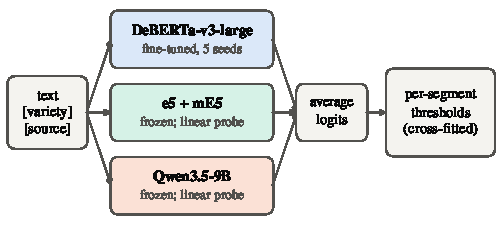
\includegraphics[width=\columnwidth]{fig_system.pdf}
\caption{The submitted system. Each of three members outputs a probability per task; we convert the probabilities to
log-odds, average them with equal weights, and apply one threshold per task and segment, fitted on out-of-fold
predictions. En-UK reviews are always labelled not sarcastic.}
\label{fig:system}
\end{figure}

The system (Figure~\ref{fig:system}) combines a fine-tuned text encoder with two classifiers trained on frozen
representations.

\paragraph{Fine-tuned encoder.} We fine-tune DeBERTa-v3-large \citep{he2023debertav} for four epochs (learning rate
$10^{-5}$, batch size 16). Each input is prefixed with its variety and source, e.g.\ \texttt{[en-UK] [reddit]}. The model
has one sentiment output and two sarcasm outputs, one for each variety. For each of the five folds we train five models
with different random seeds, and we average the predicted probabilities of the 25 models on the test set.

\paragraph{Embedding probe.} A logistic regression \citep{pedregosa2011sklearn} on concatenated sentence embeddings from
e5-large-v2 \citep{wang2022e5} and multilingual-e5-large-instruct \citep{wang2024me5}, which are not fine-tuned. The
regularisation strength is chosen by three-fold cross-validation within each training fold.

\paragraph{LLM probe.} Qwen3.5-9B \citep{qwen35}, a 9-billion-parameter LLM with weights quantised to 4 bits
\citep{dettmers2023qlora}, processes each text inside a prompt that asks whether the text is sarcastic (or positive) and
contains no labelled examples. The sarcasm prompt's definition differs by variety (Appendix~\ref{app:repro}). We train a
logistic regression, i.e.\ a linear probe \citep{alain2017probes}, on the layer-24 hidden-state vector at the last prompt
token, concatenated with the scalar difference between the logits of the ``yes'' and ``no'' answer words. Each variety has its own
sarcasm probe.

\paragraph{Combination.} We convert each member's probability to log-odds and average the three values with equal
weights. Learned weights and stacking \citep{wolpert1992stacked} did not meet our improvement criteria
(\S\ref{sec:negative}). Because only 1 of the 2,065 en-UK reviews in the pool is labelled sarcastic, the system labels
every en-UK review not sarcastic.

\section{Results}
\label{sec:results}

\begin{table}[t]
\centering\small
\setlength{\tabcolsep}{3.5pt}
\begin{tabular}{lccccc}
\toprule
 & \multicolumn{2}{c}{Sentiment} & \multicolumn{2}{c}{Sarcasm} & \\
\cmidrule(lr){2-3}\cmidrule(lr){4-5}
 & AU & UK & AU & UK & Score \\
\midrule
DeBERTa (5 seeds), OOF & .931 & .972 & .803 & .816 & .867 \\
Embedding probe, OOF & .917 & .969 & .777 & .788 & .847 \\
9B LLM probe, OOF & .916 & .973 & .789 & .806 & .853 \\
\midrule
Ensemble, OOF & .934 & .976 & .805 & .841 & .869 \\
Ensemble, \textbf{test} & .932 & .976 & .801 & .837 & \textbf{.867} \\
DeBERTa (5 seeds), \textbf{test} & .916 & .975 & .793 & .820 & .854 \\
\midrule
Organisers' baseline, test & .866 & .931 & .680 & .696 & .773 \\
\bottomrule
\end{tabular}
\caption{Macro-F1 for each task and variety; official score $=\frac12[\min(\text{sentiment AU, UK})+\min(\text{sarcasm
AU, UK})]$. OOF: out-of-fold predictions on the pool, with cross-fitted thresholds (\S\ref{sec:protocol}). The baseline is the organisers' fine-tuned DistilBERT
\citep{sanh2019distilbert,alta2026baseline}; its test scores are from the official leaderboard.}
\label{tab:main}
\end{table}

\paragraph{Test score and pre-submission estimate.} The ensemble scored 0.8668 on the test set (Table~\ref{tab:main}),
0.0025 below its OOF estimate of 0.8693. Before submitting, we computed a heuristic interval of 0.844--0.895: the OOF
score $\pm1.645$ bootstrap standard deviations, widened by 20\% as recommended by an internal review of the validation
code; its coverage is not established. Each test macro-F1 differs from the corresponding OOF macro-F1 by at most 0.004.
En-AU had the lower macro-F1 in both tasks, so en-AU set the official score. The test--OOF difference of 0.0025 is
smaller than the bootstrap standard deviation of 0.013.

\paragraph{Ranking.} Our submission ranked second, 0.0007 below the top submission. The organisers compared the top
submissions with an approximate randomisation test with 10{,}000 replicates \citep{dror-etal-2018-hitchhikers}, found no
significant differences among the top six, and declared all six joint winners \citep{alta2026task}. A non-significant
difference does not show that two submissions are equivalent, only that the test did not distinguish them. According to
the organisers, our submission and the top submission differ on 33 of the 1,573 sentiment labels (2.1\%) and 74 of the
1,573 sarcasm labels (4.7\%).

\paragraph{Effect of the probes on the test set.} To measure the contribution of the probes, we also submitted the
DeBERTa models alone. They scored 0.854, against 0.867 for the ensemble, a difference of 0.0127. The paired bootstrap on
the pool had estimated a mean gain of +0.005 (90\% interval $-$0.010 to +0.023), so the observed gain lies within that
interval. On the pool, the submitted five DeBERTa seeds scored 0.867 and the ensemble 0.869; averaged over subsets of five
seeds drawn from ten, adding the probes raises the score by 0.0067 (Figure~\ref{fig:gains}b). On the test set,
DeBERTa alone lost most in the two binding en-AU components: sentiment fell from 0.931 (OOF) to 0.916 and sarcasm from
0.803 to 0.793.

\section{Training Data, Seeds and Labels}
\label{sec:analysis}
On the screening fold, the alternative encoders we tried scored 0.009--0.016 below DeBERTa-v3-large, and none of the
additional interventions met our improvement criteria (\S\ref{sec:negative}). This section examines three factors in
turn: training-set size, seed averaging and the labels.

\begin{figure*}[t]
\centering
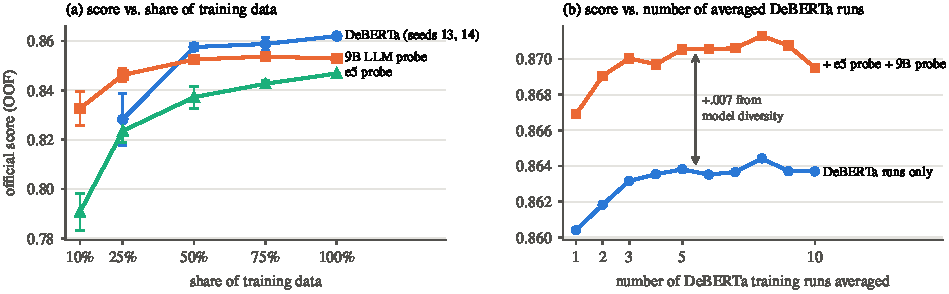
\includegraphics[width=\textwidth]{fig_gains.pdf}
\caption{Official OOF score as a function of training-set size and of the number of averaged DeBERTa runs. (a) Each
model is trained on nested subsets of every training fold, stratified by segment (DeBERTa: mean of the scores of seeds 13 and 14, evaluated separately;
probes: mean of three subset draws below 100\%; error bars: standard deviation). (b) Mean score over subsets of ten
DeBERTa runs with different random seeds (up to 30 subsets per point), alone and with the two probes added. The labelled
y-axis ticks run from 0.860 to 0.870: the 0.003 gain from one to three seeds is smaller than the 0.004 difference between two five-seed sets
of the same configuration.}
\label{fig:gains}
\end{figure*}

\subsection{Training-set size and seed averaging}
\label{sec:capacity}
\paragraph{Training-set size.} With the same two seeds (13 and 14) at every size, DeBERTa's
mean score over the two seeds is 0.858, 0.859 and 0.862
at 50, 75 and 100\% of each training fold, a gain of 0.004; the LLM probe scores 0.853, 0.854 and 0.853
(Figure~\ref{fig:gains}a). DeBERTa is trained for four epochs at every size, so smaller subsets also receive fewer
parameter updates. From 50 to 100\%, DeBERTa's Reddit sarcasm AUC rises by 0.022 in en-UK (0.845 to 0.867), which has
248 sarcastic Reddit comments in the pool, and by 0.012 in en-AU (0.833 to 0.845). The embedding probe rises from 0.837
to 0.847. For DeBERTa and the LLM probe, score gains are smaller above 50\% than below it; these curves do not estimate
the effect of data outside the pool or of models larger than 9 billion parameters.

\paragraph{Seed averaging.} Averaging DeBERTa runs with different seeds yields 0.860 for one run, 0.863 for three and
0.864 for ten (Figure~\ref{fig:gains}b). Adding the two probes raises the score by 0.0069 at three runs and by 0.0058 at
ten, more than the 0.0005 gained from three to ten runs. Two separately trained five-seed sets of the same configuration
differ by 0.004, which indicates the size of seed-to-seed variation.

\paragraph{Design choices.} We ablated three choices, evaluating predictions averaged over seeds 13 and 14 (baseline
0.865). Removing the \texttt{[variety] [source]} prefix lowers the score to 0.857 (suggestive: $\pboot=0.84$ for the
baseline; lower on 4 of 5 folds). Training two single-task models instead of one multi-task model gives 0.865
($\pboot=0.63$), and sharing one sarcasm output across varieties gives 0.863 ($\pboot=0.74$).

\subsection{Sarcasm-label rates and cue associations}
\label{sec:constructs}

\begin{figure}[t]
\centering
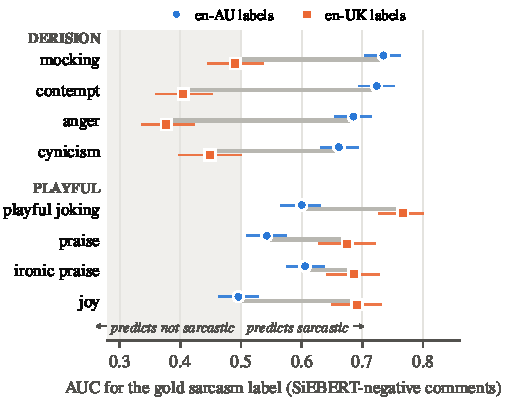
\includegraphics[width=\columnwidth]{fig_cue_flip.pdf}
\caption{ROC AUC of each derision and playful cue for the annotator's sarcasm label, among Reddit comments that SiEBERT
\citep{hartmann2023siebert} labels negative (en-AU $n=1{,}271$, 685 sarcastic; en-UK $n=912$, 186 sarcastic), with
95\% intervals from 1,000 comment-level bootstrap replicates (not adjusted for multiple comparisons). Values above 0.5:
higher cue scores among comments labelled sarcastic; below 0.5: lower.}
\label{fig:cues}
\end{figure}

The two label sets differ in the share of negative comments labelled sarcastic and in how sarcasm labels relate to
automatically scored cues. Among Reddit comments labelled sarcastic, 97\% (en-AU) and 99\% (en-UK) also carry the
negative sentiment label, but the en-AU annotator labels 60\% of comments with the negative label sarcastic, against
24\% in en-UK. The gap holds within each community: among comments that the SiEBERT sentiment classifier
\citep{hartmann2023siebert} labels negative, each of the three en-AU subreddits has a higher share labelled sarcastic
(44--64\%) than each of the four en-UK subreddits (12--33\%; Figure~\ref{fig:headline}a).

\paragraph{Derision and playful cues.} Accounts of sarcasm distinguish two components: ridicule of a target, which
separates sarcasm from irony in general \citep{lee1998ridicule}, and a positive or humorous surface that the speaker does
not mean, as in ironic praise \citep{riloff-etal-2013-sarcasm} or in jocular mockery that is not meant seriously
\citep{haugh2010jocular}. We measure each component with automatic cues. \emph{Derision cues} score whether a comment
ridicules or expresses hostility towards a target: mocking, contempt, anger and cynicism. \emph{Playful cues} score
whether it has a humorous or positive surface: joking, praise, ironic praise and joy. The first seven cues are scores
from a natural language inference (NLI) classifier \citep{laurer2023zeroshot}, which estimates whether the comment
entails short hypotheses such as ``The author is mocking someone''; joy is the probability assigned by an emotion
classifier \citep{hartmann2022emotion} (exact hypotheses in Appendix~\ref{app:repro}). Neither model was trained on
BESSTIE labels, so the cues are automatic estimates, not human judgements.

\paragraph{Associations with the sarcasm label.} We measure each cue's association with the gold sarcasm label as ROC
AUC (the probability that a randomly chosen comment labelled sarcastic has a higher cue score than a randomly chosen
comment labelled not sarcastic; Figure~\ref{fig:cues}). To avoid selecting comments by the annotator's own sentiment
labels, we use the comments that SiEBERT labels negative, and we also report AUCs on all Reddit comments. In en-AU, the
derision cues have AUCs of 0.73 (mocking), 0.72 (contempt), 0.69 (anger) and 0.66 (cynicism). In en-UK, contempt and
anger have AUCs of 0.41 and 0.38 (inverse associations); mocking has 0.49 (95\% interval 0.45--0.54) and cynicism 0.45
(0.40--0.50). The playful cues have AUCs of 0.68--0.77 in en-UK (joking 0.77, praise 0.68, ironic praise 0.69, joy 0.69)
against 0.50--0.61 in en-AU. On all Reddit comments, the derision AUCs are 0.76--0.80 in en-AU and 0.40--0.51 in en-UK.
Within each subreddit, the four derision cues have AUCs of 0.62--0.74 in all three en-AU subreddits, and contempt and
anger have AUCs of 0.33--0.47 in all four en-UK subreddits; en-UK mocking ranges from 0.37 (GreatBritishMemes) to 0.56
(unitedkingdom). The direction of the contempt and anger associations is therefore consistent across the sampled
subreddits, although the two varieties' comments come from different communities. The eight cues were chosen for
interpretability from 18 NLI-derived scores (16 hypothesis groups and 2 contrasts between them) and the emotion
classifier's outputs; the selection and comparisons are exploratory.

\paragraph{Possible explanations.} The guideline counts ``irony or mockery'' used to express contempt or ridicule. The
en-AU associations are compatible with the inclusive reading, in which literal mockery that expresses contempt counts as
sarcasm; the en-UK associations are compatible with the narrower reading, in which literal hostility alone does not.
These associations do not establish either annotator's decision rule. Possible explanations include differences between
the annotators' interpretations of the guideline; differences in how the communities use mockery, which can combine
apparent hostility with closeness \citep{haugh2012mock}; and differences between the sampled texts, since each
annotator labelled different comments. The cue scores are classifier outputs whose errors may also differ between
varieties. Because annotators and texts are not crossed between varieties, these explanations cannot be separated here;
a design in which several annotators from each variety label the same comments would allow annotator and item effects
to be estimated. Our system's prompt selection is compatible with the same difference: during development, a sarcasm
definition that includes literal ridicule raised the zero-shot LLM's en-AU Reddit sarcasm AUC from 0.65 to 0.78, and a
definition that requires non-literal meaning was kept for en-UK (Appendix~\ref{app:repro}); this choice was made on
OOF results and is not independent evidence. The difference is consistent with the lower cross-variety sarcasm
performance that BESSTIE reported. In our own experiment, averaged over three seeds, DeBERTa's Reddit sarcasm AUC on
en-AU is 0.840 when trained on en-AU and 0.678 when trained on en-UK ($-$0.162), and on en-UK it is 0.859 when trained
on en-UK and 0.715 when trained on en-AU ($-$0.144). Sentiment AUC, evaluated on both sources, falls by at most 0.011.
Training on both varieties with the variety prefix gives sarcasm AUCs of 0.845 (en-AU) and 0.861 (en-UK), against 0.840
and 0.859 for training on the evaluation variety alone. Our system uses both the variety prefix and variety-specific
sarcasm outputs; this comparison does not isolate their separate effects.

\subsection{Agreement and sarcasm discrimination in en-AU}
\label{sec:ceiling}
BESSTIE's second annotator labelled 50 items per variety \citep[\S2.3]{srirag-etal-2025-besstie}, giving Cohen's $\kappa$
(agreement corrected for chance; \citealp{cohen1960kappa}) of 0.47 for en-AU sarcasm, against 0.61 (en-AU) and 0.79
(en-UK) for sentiment; BESSTIE reports no confidence interval for these 50-item estimates. Our submitted ensemble agrees
with the gold en-AU sarcasm labels at $\kappa=0.56$ (95\% bootstrap interval 0.52--0.59) over all 2,004 en-AU Reddit
comments. The two estimates come from different samples and cannot be compared directly, and neither estimates the
highest score attainable on this task. Among Reddit comments that the annotator labelled negative, our ensemble's sarcasm
AUC is 0.77 in en-AU against 0.91 in en-UK. Our results do not distinguish whether the lower en-AU value reflects the
labelling convention, conversational context that the models do not see, or limitations of the models we tested.

\section{Interventions That Did Not Help}
\label{sec:negative}
After the three-member ensemble was fixed, none of the interventions reported in Appendix~\ref{app:negative} met its
improvement criterion. Alternative pretrained encoders (ELECTRA, ModernBERT and an NLI-tuned DeBERTa) scored 0.009 to
0.016 below DeBERTa-v3-large on the screening fold and changed the ensemble's score by $-$0.007 to +0.002. On the
screening fold, an exponential moving average of the weights changed DeBERTa's score by +0.001, layer-wise
learning-rate decay with weight averaging by +0.004, continued pre-training on unlabelled in-domain text by $-$0.004,
and preliminary training on external sarcasm data by $-$0.011. Qwen3.5-4B fine-tuned with low-rank adaptation (LoRA)
scored 0.02 below three-seed DeBERTa on the screening fold and did not change the ensemble's score. Adding recovered
thread text, features derived from the labels of other comments in the same thread, or a label vote of the 30 nearest
neighbours in the embedding space changed the score by $-$0.001, +0.001 and $-$0.005. Pseudo-labelling (training on
unlabelled texts labelled by our own models) raised the score from 0.881 to 0.886 on the screening fold but lowered it
from 0.865 to 0.859 on the confirmation fold ($\pboot=0.95$ for the baseline), so it failed its pre-specified
confirmation.

\section{Conclusion}
\label{sec:conclusion}
A three-member ensemble selected with cross-validation and paired bootstrap comparisons scored 0.867, ranked second, and
was one of six joint winners. In the label analysis, among comments labelled negative by a sentiment classifier, 44--64\%
are labelled sarcastic in each en-AU subreddit against 12--33\% in each en-UK subreddit, and contempt and anger scores
are associated with the sarcastic label in en-AU but with the non-sarcastic label in en-UK; BESSTIE reports human
agreement of $\kappa=0.47$ for en-AU sarcasm. Cross-variety performance differences on this benchmark may therefore
reflect differences in labelling conventions and texts as well as model generalisation. For our submission, en-AU had
the lower macro-F1 in both tasks, and en-AU sarcasm had the lowest test macro-F1 of the four components (0.801). On
the pool, among Reddit comments that the annotator labelled negative, our OOF sarcasm AUC was 0.77 in en-AU against
0.91 in en-UK. We suggest that benchmarks comparing varieties specify
whether literal mockery that expresses contempt or ridicule counts as sarcasm, have annotators from each variety label a
shared set of items, and report agreement per variety.

\section*{Limitations}
BESSTIE's annotators could consider conversational context that our models do not see. The exploratory LLM
re-annotation (Appendix~\ref{app:readers}) uses one model with a narrower guideline than BESSTIE's and is not evidence
of annotation error. With one annotator per variety, each labelling different comments, we cannot separate the effects
of individual annotators, communities and texts; our findings describe this dataset's labels, not Australian or British
English in general. The human agreement estimate (50 items) and our ensemble's agreement estimate (2,004 comments) come
from different samples. Our bootstrap intervals resample comments and do not model dependence between comments from the
same thread. The cue analyses are exploratory, use classifier scores as indirect measures of derision and playful
language without manual validation in each variety, and are not corrected for multiple comparisons. We did not test
models larger than 9 billion parameters, so our curves do not rule out gains from larger models. The bootstrap standard
deviation of the official score at test-set size is about 0.013, larger than most differences between configurations
that we report, so we base comparisons on OOF predictions and paired resampling. The DeBERTa epoch count was chosen on
the fold later used for screening, which may bias those screens upwards. The system always labels en-UK reviews not
sarcastic.

\section*{Ethics and Data}
Our code is released at \url{https://github.com/Sekinal/alta2026-stargazers}, and a release with predictions, cached
features and model checkpoints at \url{https://huggingface.co/Thermostatic/alta2026-thermostatic}. Neither release
contains competition texts; Table~\ref{tab:examples} contains paraphrases. For the split audit we matched Reddit comments
to a public archive and retained only subreddit names, thread identifiers and timestamps, without usernames; we do not
release this metadata. Competition texts were processed by Anthropic's models through Claude Code during development.
The LLM re-annotation received the guideline, the text, its variety and an item identifier, without gold labels or
model predictions. The GPT-6 Astra reviewers received the paper and aggregate results, not competition texts. External
data used in exploration came from public sources under the terms listed in Appendix~\ref{app:resources}; none is
redistributed.

\section*{Acknowledgements}
All code, experiments and analyses, and the first draft of every section of this paper, were produced by Claude Code \citep{claudecode},
running Claude Opus~5 and Claude Opus~5.5, under the author's direction; sub-agents of the same model also served as the blind
readers (Appendix~\ref{app:readers}) and as internal reviewers, and OpenAI's GPT-6 Astra, run through the Codex
CLI, reviewed the paper independently in several rounds. The design drew on the author's experience in Kaggle
competitions, including recipes adapted from the author's earlier AstroCLIMB system, and on a ChatGPT-generated list
of LoRA variants with links to their papers that the author supplied; the agents contributed the ensemble, output-head,
prefix and probe designs from their prior knowledge. The sarcasm and annotation literature was read after the system was
fixed and did not change it. A full account of the development process, including mistakes found
and corrected, is released with our code. The author reviewed and edited the paper and takes full
responsibility for its content; AI systems are not authors of this work. We thank Lium for a generous grant of GPU
credits that made this and other work possible, and the organisers, Diego Moll\'{a}-Aliod, Aditya Joshi and Dipankar
Srirag, for running the shared task and for their careful significance analysis.

\bibliography{references}

\appendix

\section{Results of Additional Interventions}
\label{app:negative}
Table~\ref{tab:negative} lists the interventions we evaluated after the three-member ensemble was fixed, under the
protocol of \S\ref{sec:protocol}. $\Delta$ is the intervention's official score minus its baseline's. One-fold DeBERTa
changes compare predictions averaged over the same three seeds; LoRA changes compare mean scores over two seeds; five-fold
changes compare OOF scores on the full pool.

\begin{table}[!ht]
\centering\small
\begin{tabular}{>{\raggedright\arraybackslash}p{4.85cm}r}
\toprule
Intervention (protocol) & $\Delta$ \\
\midrule
\multicolumn{2}{l}{\emph{DeBERTa training / encoder} (one fold, same 3 seeds)} \\
\quad weight averaging (EMA) & +.001 \\
\quad layer-wise learning-rate decay + EMA & +.004 \\
\quad NLI-tuned DeBERTa-v3-large & $-$.016 \\
\quad ELECTRA-large & $-$.009 \\
\quad ModernBERT-large & $-$.012 \\
\quad any of these added to the ensemble & $-$.007 to +.002 \\
\quad continued in-domain pre-training & $-$.004 \\
\quad sarcasm pre-training (external data) & $-$.011 \\
\midrule
\multicolumn{2}{l}{\emph{LLMs} (Qwen3.5-4B \citealp{qwen35}, one fold)} \\
\quad LoRA + rsLoRA, alone / in ensemble & $-$.02 / .000 \\
\quad EVA + rsLoRA & $-$.04 \\
\quad EVA + DoRA + rsLoRA + Riemannian & $-$.10 \\
\midrule
\multicolumn{2}{l}{\emph{Data and context} (five folds unless noted)} \\
\quad pseudo-labels (pre-spec., fold 4) & $-$.006 \\
\quad recovered thread text (stacked) & $-$.001 \\
\quad same-thread label features & +.001 \\
\quad 30-nearest-neighbour label vote & $-$.005 \\
\quad LLM label as feature, en-UK (pre-spec.) & .000 \\
\bottomrule
\end{tabular}
\caption{Change in official score against the matching baseline (DeBERTa rows and LoRA alone: three-seed DeBERTa on the
same fold; LoRA variants: LoRA + rsLoRA; pseudo-labels: the unchanged ensemble on fold 4; other five-fold rows: the full ensemble, or for thread context the same
second-stage classifier without the thread features). Pre-spec.: evaluated against a criterion written before the
run. Methods: exponential moving average of the weights (EMA); layer-wise learning-rate decay
\citep{howard-ruder-2018-universal}; NLI-tuned DeBERTa \citep{laurer2024less}; ELECTRA \citep{clark2020electra};
ModernBERT \citep{warner2024modernbert}; continued in-domain pre-training \citep{gururangan-etal-2020-dont}; sarcasm pre-training data (Appendix~\ref{app:resources}); low-rank adaptation (LoRA; \citealp{hu2022lora}) with rank-stabilised scaling (rsLoRA;
\citealp{kalajdzievski2023rslora}), explained-variance initialisation (EVA; \citealp{paischer2024eva}), weight-decomposed
LoRA (DoRA; \citealp{liu2024dora}) and Riemannian preconditioning \citep{zhang2024riemannian}, implemented with the PEFT
library \citep{peft} (the EVA initialisation was capped at 32 batches and had not converged in 115 of 248 layers); pseudo-labelling
\citep{lee2013pseudo}, following a recipe from the author's earlier AstroCLIMB system. For the alternative encoders, sarcasm pre-training, the LoRA variants and pseudo-labelling (0.95), $\pboot$ for the
baseline is at least 0.8; no intervention reaches $\pboot\geq0.8$ over its baseline.}
\label{tab:negative}
\end{table}

\section{Exploratory LLM Re-annotation}
\label{app:readers}
We asked whether an LLM annotator without access to the gold labels would reproduce them. Two separate runs of Claude
Opus~5.5 labelled the same 399 Reddit comments: 150 sampled uniformly per variety, plus 50 en-AU and 49 en-UK comments
whose OOF ensemble probability differed from the gold sarcasm label by more than 0.8. Each run received the comments in
shuffled batches of 100, with the text, its variety and an item identifier but no labels or predictions, and this
guideline: ``You are annotating short Reddit comments from Australian (en-AU) or British (en-UK) English speakers. For
each item give two labels, judging the text as written (you do not see the thread it came from): sarcasm: 1 if the author
says something they do not literally mean in order to mock, criticise, or be ironic/teasing (sarcasm, verbal irony, mock
praise, rhetorical ridicule); 0 otherwise. Plain complaints, jokes that are not ironic, and sincere statements are 0.
sentiment: 1 if the overall attitude/emotion expressed is positive, 0 if it is negative (or neutral-leaning negative).''
This guideline is narrower than BESSTIE's: it requires non-literal meaning and counts plain complaints as not
sarcastic. The sample, guideline and criteria were written before annotation and committed to version control together with the
results.

\begin{table}[!ht]
\centering\small
\setlength{\tabcolsep}{3pt}
\begin{tabular}{lcccc}
\toprule
 & G--O & G--R & O--R & Positive rate G / O / R \\
\midrule
Sarc AU & \textbf{.56} & .21--.28 & .30--.34 & .43 / .43 / .16 \\
Sarc UK & .59 & .62 & .45 & .29 / .23 / .27 \\
Sent AU & .74 & .60--.65 & .60--.65 & .29 / .33 / .26 \\
Sent UK & .85 & .81--.83 & .67--.69 & .17 / .15 / .22 \\
\bottomrule
\end{tabular}
\caption{Agreement (Cohen's $\kappa$, \citealp{cohen1960kappa}) on 150 random Reddit comments per variety between the gold
labels (G), our ensemble (O) and the two readers (R; ranges over readers), and the share each labels positive (sarcastic,
or positive sentiment; R is the mean of the two runs). 95\% bootstrap intervals for G--O sarcasm: 0.43--0.70 (en-AU)
and 0.44--0.72 (en-UK).}
\label{tab:reannot}
\end{table}

\paragraph{Results.} The two runs agree with each other at $\kappa=0.90$ (en-AU) and 0.97 (en-UK) for sarcasm and 0.91
and 0.98 for sentiment. This measures agreement between repeated runs of one model, not agreement with independent human
judgements. LLM labels can also differ systematically from human judgements on subjective
tasks \citep{pavlovic-poesio-2024-effectiveness}. In the uniform samples, 43\% of en-AU comments are labelled sarcastic
in the gold data against 16\% by the LLM runs (mean), and 29\% against 27\% in en-UK (Table~\ref{tab:reannot}). Our
ensemble agrees with the gold en-AU sarcasm labels at $\kappa=0.56$ and with the two runs at 0.30 and 0.34.

\paragraph{Pre-specified criteria.} We wrote down three criteria for the hypothesis that label
disagreement limits further gains: (i) the two runs agree with
each other more than with gold (met); (ii) our ensemble agrees with the runs at least as much as with gold (not met in
either variety); (iii) on the disputed comments where the runs agree, they agree with our ensemble more than 60\% of the
time (met: 31 of 45 en-AU, 31 of 48 en-UK). Criterion (iii) does not distinguish agreement with the ensemble from a
preference for the non-sarcastic label: on en-AU comments the runs choose the non-sarcastic label in
28 of 32 cases where the ensemble gives it and in 10 of 13 cases where the gold label gives it. On en-UK comments they
agree with the ensemble in 26 of 42 and 5 of 6 such cases. The pre-specified evidence therefore
does not establish that label disagreement limits further gains. Adding a reader's label to the ensemble as a pre-specified en-UK feature
raised en-UK Reddit sarcasm AUC from 0.906 to 0.920 and en-UK sarcasm macro-F1 from 0.841 to 0.843, but left the official
score unchanged, because en-AU remained the binding variety.

\paragraph{Limitations of the re-annotation.} Both runs used one LLM, from the model family used to develop our system,
with a stricter definition than BESSTIE's; they are not judgements by speakers of either variety. The lower en-AU rate
(16\% against 43\%) may reflect the stricter definition, a model that does not recognise jocular mockery and abuse,
which have been described in Australian and British interaction \citep{haugh2012mock}, or the annotator's convention;
we cannot separate these. The analyses in the main text do not use these labels.

\section{Reproducibility Details}
\label{app:repro}
\paragraph{Folds and thresholds.} Five folds over the pool (fold-assignment seed 2026), stratified by segment and both labels, with
identical texts kept in one fold. Thresholds: one per task and segment, chosen by coordinate ascent (one threshold at a
time) to maximise the macro-F1 of the corresponding task and variety; en-UK reviews are always labelled not sarcastic. Reported OOF scores fit thresholds on four
folds and apply them to the fifth; test thresholds are fitted on all OOF predictions.

\paragraph{Ensemble.} On the test set, the DeBERTa member's probability is the mean over its 25 models (5 seeds
$\times$ 5 folds); for OOF predictions it is the mean over the five seeds trained without the text's fold. Each probe's
test probability is the mean over its five fold models. With $\ell(p)=\log\frac{p}{1-p}$ and
$\sigma(z)=1/(1+e^{-z})$, the ensemble probability is $\sigma\big(\tfrac13[\ell(p_{\mathrm{DeB}})+\ell(p_{\mathrm{e5}})
+\ell(p_{\mathrm{LLM}})]\big)$.

\paragraph{DeBERTa.} The first token's final hidden state feeds one sentiment output and two sarcasm outputs, one per
variety (the text's variety selects the sarcasm output); loss = binary cross-entropy for sentiment + binary cross-entropy for sarcasm, equal weights;
AdamW \citep{loshchilov2019adamw}, learning rate $10^{-5}$, batch 16, linear warmup over the first 10\% of steps, bfloat16 arithmetic, 4 epochs, maximum length 256 tokens (longer texts keep
head and tail); seeds 13--17.

\paragraph{Embedding probe.} e5-large-v2 embeddings with the prefix ``query: '' are concatenated with
multilingual-e5-large-instruct embeddings computed with the instruction ``Decide whether the given online review or
comment is sarcastic or ironic''; features are standardised and a logistic regression is fitted per task, with $C$
chosen by three-fold inner cross-validation.

\paragraph{LLM probe.} Qwen3.5-9B with 4-bit NormalFloat (NF4) weights (double quantisation, bfloat16 arithmetic), using its chat template
with the reasoning mode disabled.
Features: the layer-24 hidden state at the last prompt token, plus the logit margin between the answer words
(case variants pooled by log-sum-exp); standardised; logistic regression (inverse regularisation strength $C=0.002$), with one sarcasm probe per
variety. The prompt names the text type (e.g.\ ``a Reddit comment from an Australian community (Australian
English)''), gives a definition and asks ``Is the text sarcastic? Answer Yes or No.'' The en-AU definition reads:
``Sarcasm here is understood broadly: the writer uses irony, mockery, ridicule, cynical or derisive jabs, snark, or
says something they do not literally mean, usually to criticise or show contempt (for example cynical remarks about
politicians, parties or government). A sincere, neutral, informative or friendly text is NOT sarcastic.'' The en-UK
definition reads: ``Sarcasm means the writer says something they do not literally mean, usually the opposite, in order
to mock, criticise or show contempt. [\ldots] A text that is merely angry, negative, rude or critical but says exactly
what it means is NOT sarcastic. British sarcasm is often dry and understated [\ldots]''; the elided parts list example forms and phrases. The sentiment prompt asks whether the overall sentiment is positive or negative and states that
sarcastic praise counts as negative. Full prompts are in the release.

\paragraph{Cue scores.} Each NLI cue is the mean entailment log-odds of \path{MoritzLaurer/deberta-v3-large-zeroshot-v2.0}
over two or three hypotheses, with the comment as premise (256 tokens, head and tail): \emph{mocking}: ``The author is mocking
someone.'', ``The author is ridiculing something.'', ``This text makes fun of someone.''; \emph{contempt}: ``The author
is contemptuous.'', ``The author looks down on someone.''; \emph{anger}: ``The author is angry.'', ``The author is
frustrated.'', ``The author is annoyed.''; \emph{cynicism}: ``The author is cynical.'', ``The author expects things to
go badly.''; \emph{playful joking}: ``The author is joking.'', ``This text is meant to be funny.'', ``The author is
being playful.''; \emph{praise}: ``The author is praising something.'', ``The author is happy with something.'', ``This
is a compliment.''; \emph{ironic praise}: ``This is ironic praise.'', ``The author pretends to be positive but is
actually negative.'', ``The compliment in this text is not meant seriously.'' \emph{Joy} is the emotion classifier's
joy probability. The other nine NLI hypothesis groups (opposite meaning, sincerity, complaint, politics, exaggeration,
rhetorical question, positive, negative, advice) and two contrasts (praise minus complaint, sincerity minus opposite
meaning) were not used as cues; we chose the eight shown as interpretable
markers of derision and play, and the selection is exploratory. AUC intervals use 1,000 comment-level bootstrap
replicates.

\section{Resources}
\label{app:resources}
\raggedright
\paragraph{Final system.} \path{microsoft/deberta-v3-large} \citep{he2023debertav}; \path{intfloat/e5-large-v2}
\citep{wang2022e5}; \path{intfloat/multilingual-e5-large-instruct} \citep{wang2024me5}; \path{Qwen/Qwen3.5-9B}
\citep{qwen35} with bitsandbytes 4-bit (NF4) quantisation \citep{dettmers2023qlora}; PyTorch \citep{paszke2019pytorch},
Transformers \citep{wolf-etal-2020-transformers}, sentence-transformers \citep{reimers-gurevych-2019-sentence} and
scikit-learn \citep{pedregosa2011sklearn}; data processing with Polars \citep{polars} and figures with Matplotlib
\citep{hunter2007matplotlib}. Trained only on the shared-task training and development data. Checkpoints screened in
Table~\ref{tab:negative}: \path{google/electra-large-discriminator}, \path{answerdotai/ModernBERT-large},
\path{MoritzLaurer/DeBERTa-v3-large-}\linebreak[0]\path{mnli-fever-anli-ling-wanli} and \path{Qwen/Qwen3.5-4B}.

\paragraph{Analyses.} \path{MoritzLaurer/deberta-v3-large-zeroshot-v2.0} \citep{laurer2023zeroshot},
\path{siebert/sentiment-roberta-large-english} \citep{hartmann2023siebert} and
\path{j-hartmann/emotion-english-distilroberta-base} \citep{hartmann2022emotion} for the cues of Figure~\ref{fig:cues};
Reddit thread metadata matched through Arctic Shift \citep{arcticshift} for the split audit.

\paragraph{External data in the reported negative results.} The sarcasm pre-training of Table~\ref{tab:negative}
used Reddit comments tagged \texttt{/s} (tag removed) from about 25 AU and 25 UK subreddits, collected through Arctic
Shift, ConvoKit's per-subreddit corpora \citep{chang-etal-2020-convokit} and the UK subreddit dumps of
\citet{redditusuk}, with untagged comments from the same subreddits as negatives; it added EPIC \citep{frenda-etal-2023-epic},
iSarcasmEval \citep{abu-farha-etal-2022-semeval}, SemEval-2018 Task~3 \citep{van-hee-etal-2018-semeval}, FigLang 2020
\citep{ghosh-etal-2020-report} and \citet{wallace-etal-2014-humans}. Domain-adaptive pre-training and pseudo-labelling used
unlabelled in-domain text: AU and UK Reddit via Arctic Shift (Reddit's terms), Google Local reviews
\citep{he2017translation,pasricha2018translation}, Booking.com reviews (\path{huggingface.co/datasets/Booking-com/accommodation-reviews}, CC BY-SA 4.0), NHS GP reviews
(\path{huggingface.co/datasets/janduplessis886/england-nhs-gp-reviews}, Open Government Licence) and Inside Airbnb
reviews (\path{insideairbnb.com}, CC BY 4.0). All external data were deduplicated against the task data, and none is used by
the final system.

\paragraph{Other exploration.} We also screened other encoders, embedding models, LLMs, zero-shot feature models and
classical models (TF-IDF, SVMs, gradient-boosted trees), and collected further sarcasm and sentiment corpora. None
contributed to the final system or to any result reported here; the release lists them all with their sources.

\end{document}
